\begin{Figure}[h]
    \centering
    \footnotesize

    \psfrag{cu}[r][r] {$\text{copper}$}
    \psfrag{alu}[l][l] {$\text{aluminum}$}
		
		\psfrag{cur1}[r][r] {$\text{current}$}
		\psfrag{col1}[r][r] {$\text{collector}$}
		
		\psfrag{cur2}[l][l] {$\text{current}$}
		\psfrag{col2}[l][l] {$\text{collector}$}
    \psfrag{ch}[c][c] {$\text{charging}$}
		\psfrag{ca}[c][c] {$\text{solid cathode}$}
		\psfrag{an}[c][c] {$\text{solid anode}$}
		\psfrag{el}[c][c] {$\text{solid electrolyte}$}
		
		
		\psfrag{z}[c][c] {$\text{LLZO}$}
		\psfrag{mlo}[c][c] {$\text{metal-oxided}$}
		
		\psfrag{gr}[c][c] {$\text{Li}+$}
		\psfrag{mo}[c][c] {$\text{metal-oxide}$}
    \psfrag{em}[c][c] {$\text{e}-$}
		\psfrag{sei}[c][c] {$\text{space charge layer}$}
		
		\psfrag{s}[c][c] {$\text{Li-metal}$}
		\psfrag{dd}[c][c] {$\text{dendrite}$}
    
		\psfrag{mn}[c][c] {$-$}
		\psfrag{pl}[c][c] {$+$}
		\psfrag{fb}[c][c] {$\mathlarger{\mathlarger{\text{\faBolt}}}$}
		
		%\includegraphics[scale=0.3]{batt.eps}te
    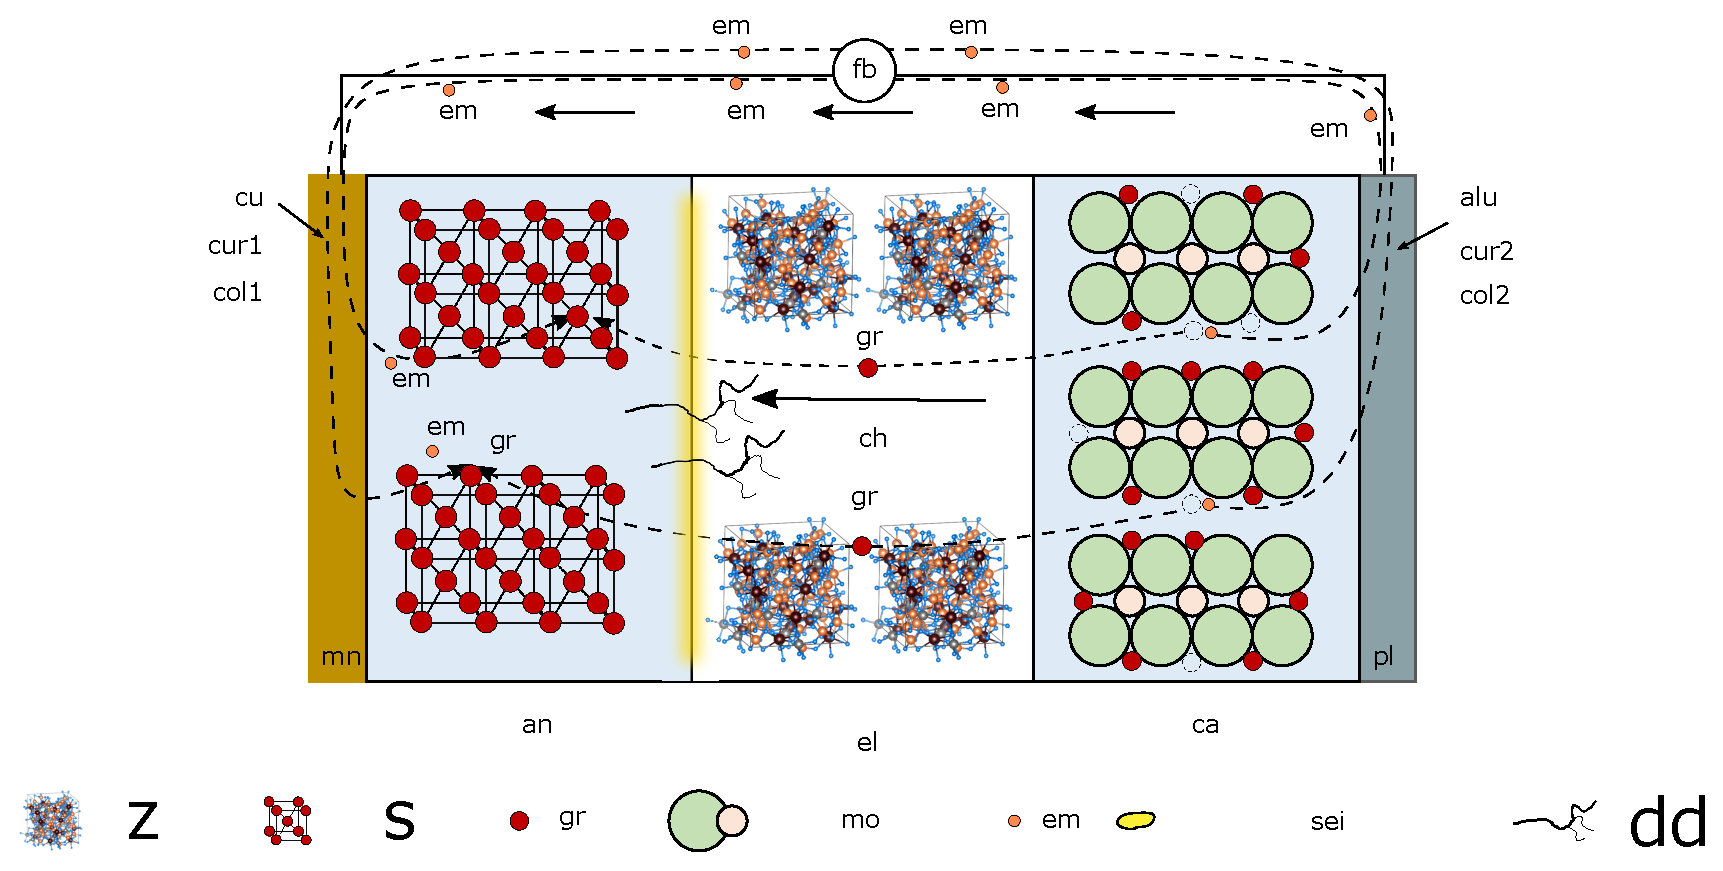
\includegraphics[width=0.65\textwidth]{transport.eps}
    %\caption{Swelling mechanism: formation of Solid Electrolyte Interphase (SEI) $\text{\faBatteryFull} \rightarrow \text{\faBatteryThreeQuarters}$. When SEI at the interphase between graphite anode and separator develops dendrites beyond half of separator towards cathode, short-circuit happens and ignite the flammable electrolyte solution. Overcharging and tiny metal impurity during manufacturing process are the two main reasons as stated by \textsc{Cui} from \textsc{Schwartz} \cite{markstanford}.}
    %\label{\LABEL}
		
\end{Figure}


